\section{Behavior Trees}
\subsection{Synopsis}
Behavior Trees are Directed Acyclic Graphs that are used to represent an agent's decision process. From a syntax perspective, they're usually represented as a tree structure constructed from multiple nodes representing various internal constructs. Each node has a return status, commonly: Success, Failure or Running, used to determine a result (or lack of one, in case of Running status) of the node's execution \cite{ksheperthesis}.  In turn, said nodes' function is to either redirect a flow of a process or to represent a decision resulting from one.
Consequently, we can derive three kinds of these nodes:
\begin{itemize}
    \item \textbf{Action} nodes reside exclusively in leaves of a tree and are, as mentioned above, a resulting decision, a set of instructions for the agent to execute. The degree of granularity is arbitrary - one can imagine both \textit{Move Forward by 1 meter} and \textit{Perform Engine Repair} to be examples of Action nodes, with relevant code belonging to Agent's implementation. Alternatively, Action nodes might point to further decision processes: for instance, \textit{Perform Engine Repair} could be a complicated procedure with separate Behavior Tree, detailing diagnostic and the actual repair.
    \item \textbf{Composite} nodes, however, are tasked with controlling how the tree is actually executed. For the purposes of this thesis, Selectors, Sequences, Parallel-All and Parallel-One types will be considered and reviewed. Note that although the ones are arguably the most widely used, many more Composite nodes types exist, fitting various use cases.
    \item \textbf{Condition} nodes are used to query a specific property of the environment, testing an internal condition and returning Success or Failure applicably - representing, in this case, True and False.
\end{itemize}
While selection of  Action and Condition nodes are (often) entirely implementation-dependent, as they must be programmed to perform specific tasks (or query the environment for specific condition), most of the Composite nodes are not dependent on the platform and may be freely reused (with the possible exception in Parallel type nodes).

\subsection{Composite Node Types}
In order to remain relatively simple to work with while maintaining versatility, flow-control nodes are possible to employ. These come in many varieties and often can be said to mimic (or at least resemble in action) logic functions.
\begin{itemize}
    \item \textbf{Sequence} nodes will test its child nodes in defined order -  executing them from left to right is the common practice, although introducing a different metric (for example, task priority) is possible \cite{ksheperthesis}. Sequence node will return Success if and only if all of its children return Success, and Failure otherwise. In this, Sequence works identically to logical AND function.
    \item \textbf{Selector} node, for all intents and purposes, is a operational opposite of Sequence. Execution order remains unchanged (along with all modification possibilities), but Selector node will return Success immediately when one of its children return Success and Failure only when all of its children return Failure. Analogically, Selector is a Behavior Tree counterpart to logical OR function.
\end{itemize}
Finally, \textbf{Parallel-One} and \textbf{Parallel-All} nodes introduce concurrence to Behavioral Trees: execution of all child tasks is simultaneous, the node returning when any (in case of Parallel-One) task or all of them (Parallel-All) return Success.

\subsection{Behavior Tree Example}
Consider the task of getting to a room through the door. For this, a behavior tree depicted in Figure \ref{fig:x btexample} was proposed (adapted from \cite{ksheperthesis}):
\begin{figure}[h]
\centering
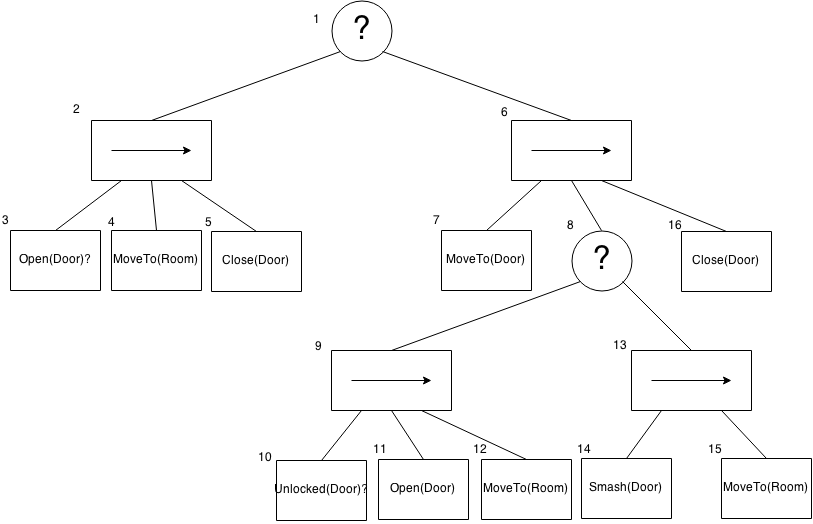
\includegraphics[scale=0.5]{btexample}
\caption{An example Behavior Tree}
\label{fig:x btexample}
\end{figure}
\newpage
In the above tree consider:
\begin{itemize}
    \item nodes 1 and 8 to be Selectors
    \item nodes 2, 6, 9 and 13 to be Sequences
    \item nodes 3 and 10 to be Conditions
    \item nodes 4, 5, 7, 11, 12, 14, 15 and 16 to be Actions
\end{itemize}
Both Action and Condition nodes here have parameters (Door and Room, which we consider constants denoting, respectably: door in question that we need to get through and a room behind it).

In case when the door is already open, Selector 1 will go to node 2 (Sequence) and, after verifying that the Door is open (Condition 3), will proceed to going through it and closing them afterwards (Actions 4 \& 5).

In case when the door is closed, but not locked, Selector 1 will go to node 2 as well, but since Condition 3 will fail, next node evaluated will be Sequence 6. After moving to the door (Action 7) we first(Sequence 9) confirm that the door is, in fact, unlocked (Condition 10) and proceed to open it and move to the room (Actions 11 and 12). After returning from Sequence 9 (with Success) and Selector 8 (since 9 returned Success), it will proceed to closing the door (Action 16).

Finally, if the door is both closed AND locked, Selector 1 will go to node 2 first, but since Condition 3 will fail, next node evaluated will be Sequence 6. After moving to the door (Action 7) and finding out that the door is locked (Condition 10), we will go straight to Sequence 13, first smashing the door (Action 14), then moving to the room (Action 15) and eventually, after returning from nodes 13 and 8, closing the door (Action 16).
\section{Genetic Algorithms}
\subsection{Motivation and History}
Genetic Algorithms are a family of search algorithms directly inspired by Charles Darwin's theory of evolution. His influential book, ``On the Origin of Species''(1859) led to a birth of the term ``survival of the fittest'' by Herbert Spencer (``Principles of Biology'', 1864), who understood it as \enquote{(\ldots) the preservation of favoured races in the struggle for life}.

Over the years, many scientists proceeded to capitalize on that phrase, designing algorithms in which potential solutions' quality (\textit{fitness}) was the deciding factor in deciding if they survive to the next round of choosing. % include citations to early works?

Genetic Algorithms' births and growth into a popular search heuristic was largely due to John Holland's ``Adaptation in Natural and Artificial Systems''. In his book, he proposed a method to apply an evolutionary process in nature to artificial systems by genetically breeding populations of fixed-length character strings (posing as solutions to a given problem) using Darwinian natural selection model and genetic operation of recombination. He was also able to conclude the following about the model problem in the book (a multi-armed slot machine)\cite{kozagp}:
\begin{quote}
   (\ldots) the genetic algorithm is a near optimal approach to adaptation in that it maximizes expected overall average payoff when the adaptive process is viewed as a multi-armed slot machine problem requiring an optimal allocation of future trials given currently available information.
\end{quote}
In following years, and after introducing some modifications, the method evolved into a shape summarized below.
\subsection{Synopsis}
The Genetic Algorithm process starts with generating a population of specimen: candidate solutions to the problem. They are then graded using user-specified, problem-specific \textit{fitness function}, and a fitness value is bound to each solution. Afterwards, the process of creating a next generations starts: specimen, based on their fitness, are chosen to be parents to new solutions. Children resulting from such union have a combination of genes from both parents, although the exact algorithm varies between different \textit{crossover} operation implementations. The children are produced until a new population's size is equal to the previous one. Additionally, new population is then subject to a process of \textit{mutation}, meaning that each child has a chance to have parts of his genes changed; this introduces some variation in the population as well as helps breaking out of local optima and broadening the search space \cite{Luke2013Metaheuristics}. With all steps finished, the whole process (sans the random initialization part) repeats until an end condition is met.

Genetic Algorithm can be thus summarized with following series of steps:
\begin{description}
    \item[Initialisation] -- start by producing (randomly or otherwise) a population of candidate solutions.
    \item[Evaluation] -- assign each specimen in current generation a fitness value determined by fitness function.
    \item[Recombination] -- choose (using chosen selection method) two parents and combine their genes in \textit{crossover} process, producing two children. Repeat until new generation is equal in size with parents' generation.  % breeding? Reproduction?
    \item[Mutation] -- subject current population to a \textit{mutation} process providing a chance to change individual genes of a specimen.
\end{description}

Furthermore, one has to make several key decisions during preparation to using Genetic Algorithms. These are commonly (after \cite{kozagp}):
\begin{description}
    \item[specimen representation] -- a mapping of the solution information to a data structure handled by the algorithm.
    \item[population size] -- number of specimen in each population.
    \item[fitness function] -- a function to assess the value of the specimen.
    \item[number or generations] -- an amount of iterations to execute before the process is finished.
    \item[additional end-conditions] -- an early option (or options) for early termination of the algorithm.
    \item[selection method] -- a strategy to choose parents for the next generation.
    \item[crossover and mutation methods] -- an exact implementation of genetic operators.
    \item[mutation and crossover rates] -- a rate by which said genetic operators affect the population.
\end{description}

Selection, Crossover and Mutation strategies have a great deal of influence over the algorithm's result and will be discussed further in sections below.
\subsection{Selection}
Selection process is a entry point to the recombination process - it's here where two specimen are chosen from the population pool to either be copied to the next generation, or become parents to (traditionally) two children, which are then added to a it instead (parents, however, are "returned" to the old one, able to be selected again). Therefore, candidates should be seen as individuals competing for a possibility to extend their lineage and pass their genes on to the next generations. Following Darwinian law, individuals with higher fitness value associated to them should have the higher chance to be selected - that was the original premise behind \textbf{Fitness Proportionate Selection}, largely popular during early developements of Genetic Algorithms \cite{Luke2013Metaheuristics}.

In \textbf{Fitness-Proportionate Selection}, also known as \textbf{Roulette selection} \cite{Luke2013Metaheuristics} specimen are selected in proportion to their fitness: solutions with higher fitness value associated have a bigger chance of being selected. Not only does it introduce an element or chance, in contrast to methods like \textbf{Elitism} or \textbf{Truncation Selection} \cite{Luke2013Metaheuristics}, where one simply copied \textit{n} best specimen (repeating that operation until new population was the right size), it also doesn't restrict the option of ``weak'' individual being selected to carry through genetic material that potentially can prove to be interesting in future. Using Roulette Selection, however, one makes a big assumption:
\begin{quote}
They presume that the actual fitness \textit{value} of an individual really means something important. But often we choose a fitness function such that higher ones are ``better'' than smaller ones, and don't mean to imply anything more.
\end{quote} \cite{Luke2013Metaheuristics}.
This can pose a significant problem during later iterations of the algorithm, when most of the solutions may have similar fitness values, effectively turning a theoretically fitness-proportional choice to strategy only slightly better then random one.

\textbf{Tournament Selection} deals with that problem in a curious way - instead of considering the fitness function values, it merely takes into consideration the ordering. The algorithm is definitely on the simpler side: a random sample of the population is chosen, and the best individual in that sample is returned as a result (hence the ``tournament''). That invulnerability on fitness function's particulars, along with the simplicity are some of the reasons why Tournament Selection has become the primary selection technique used for Genetic Algorithm \cite{Luke2013Metaheuristics}. Furthermore, this method offers additional great advantage - its behavior easily adjustable. By setting a tournament size small, for instance, one can expect it to be less \textit{selective}, since ``weaker'' individuals might still win in smaller instances of the tourney. By setting it to a large value, one can expect the method to strongly prefer top performers. Setting it to a \textit{too large} value, however, will guarantee that the new population will be constructed from one specimen.

\subsection{Crossover}
Unlike other evolution-inspired techniques, in GA selected individuals are not always explicitly copied to the next generation. Instead, selected individuals have a chance (dictated by \textbf{crossover rate}) to undergo a process that will recombine their genes in order to form two offspring (although a research by Eiben et al., 1994 mentioned in \cite{ksheperthesis} suggests that using more than two parents might generate higher quality children). The common method of doing that seems to be One- or Multi Point Crossover, which involves choosing a random point (points) along each specimen representation and exchanging genetic material between them. Figure \ref{fig:x crossoverexample} illustrates the process of One- and Two-Point Crossover operations.
\begin{figure}[h]
    \centering
    \begin{subfigure}[b]{0.5\textwidth}
        \centering
        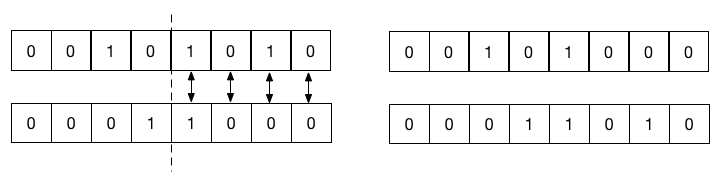
\includegraphics[width=\textwidth]{crossover}
        \caption{One-Point Crossover}
        \label{fig:onepointcrossover}
    \end{subfigure}
    \hfill
    \begin{subfigure}[b]{0.5\textwidth}
        \centering
        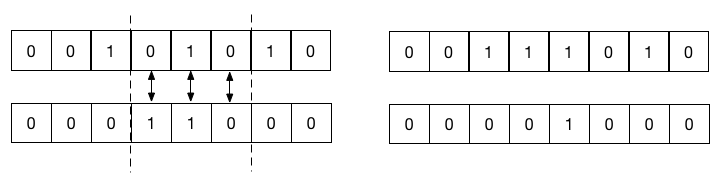
\includegraphics[width=\textwidth]{crossover2}
        \caption{Two-Point Crossover}
        \label{fig:twopointcrossover}
    \end{subfigure}
    \caption{Crossover Example}
    \label{fig:x crossoverexample}
\end{figure}
In some cases crossover might prove to be quite a destructive force. Namely, it has to do with \textit{linkage} (or \textit{epistasis}) between elements in specimen representation \cite{Luke2013Metaheuristics}. Elements that are feasible in current setting might, and will be, broken up, and one can easily imagine crossover operation producing a number of ``broken'' or otherwise flawed individuals.

\subsection{Mutation}
Mutation operation serves as an assurance that the algorithm won't converge prematurely by introducing that much-needed variance. It's usually performed on a whole population, where each individual has a chance of his genes randomly changing (provided by \textbf{mutation rate}). Depending on the actual representation of the chromosome, popular implementations include a bit-flip (in case of boolean strings, for example) or replacing a value with one randomly generated with given distribution.
\section{Genetic Programming}
\subsection{Motivation}
John R. Koza, creator of Genetic Programming, wrote the following on motivation and scope of this field \cite{kozagp}:
\begin{quote}
    The genetic programming paradigm continues the trend of dealing with the problem of representation in genetic algorithms by increasing the complexity of the structures undergoing adaptation. In particular, the structures undergoing adaptation in genetic programming are general, hierarchical computer programs of dynamically varying size and shape.(\ldots)
I claim that the process of solving these problems can be reformulated as a search for a highly fit individual computer program in the space of possible computer programs. When viewed in this way, the process of solving these problems becomes equivalent to searching a space of possible computer programs for the fittest individual computer program.
\end{quote}

\subsection{Key Differences}
Apart from the issue of representation, Genetic Programming is, in its essence, merely an adaptation of Genetic Algorithm, with further changes to accommodate handling of a different data structure. As such, only said changes will be described here, while the remaining parts of the algorithm are assumed to be unchanged. Note here that in interest of convenience, all examples below have been presented on Behavior Tree structures.
\subsubsection{Crossover}
Crossover works in similar way to its Genetic Algorithm counterpart, selecting a random nodes in each parent and exchanging them (along with their respective subtrees). Figure \ref{fig:x gpcrossoverexample} illustrates two specimen before and after crossover procedure.
\begin{figure}[h]
    \centering
    \begin{subfigure}[b]{0.5\textwidth}
        \centering
        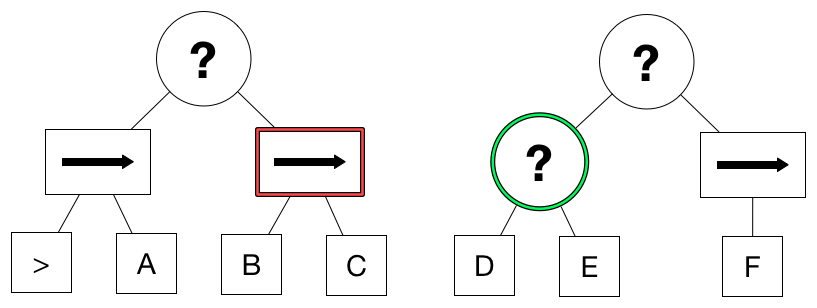
\includegraphics[width=\textwidth]{gpcrossover}
        \caption{Step 1: selecting nodes to be exchanged.}
        \label{fig:gpcrossover1}
    \end{subfigure}
    \hfill
    \begin{subfigure}[b]{0.5\textwidth}
        \centering
        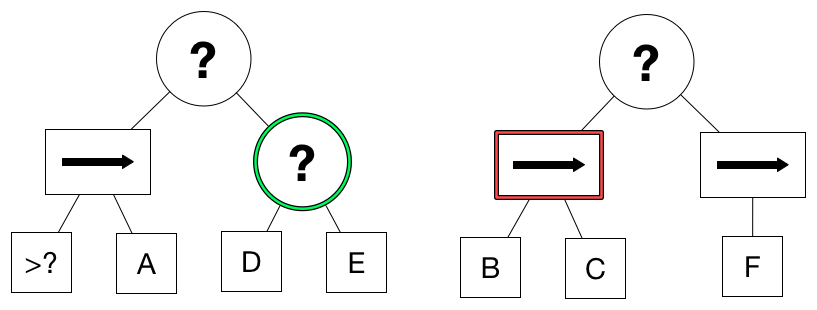
\includegraphics[width=\textwidth]{gpcrossoverres}
        \caption{Step 2: performing the exchange.}
        \label{fig:gpcrossover2}
    \end{subfigure}
    \caption{Crossover Example}
    \label{fig:x gpcrossoverexample}
\end{figure}
\subsubsection{Mutation}
Changes to mutation, however, took a more significant turn. Genetic Programming mutation is defined in two ways: one still could be rather similar to Genetic Algorithm mutation (\textbf{micromutation}). The other one, called \textbf{macromutation} (or \textbf{``Headless Chicken''} ) is an entirely new way of introducing variance to a population. While micromutation consists of randomly selecting a node in a tree and changing its parameters, macromutation is executed by replacing a random node with a new, randomly-generated, tree - in certain cases, it may result in replacing the whole tree. Figures \ref{fig:x gpmicromutationexample} and \ref{fig:x gpmacromutationexample} present an example of performing micro- and macromutation.
\begin{figure}[h]
    \centering
    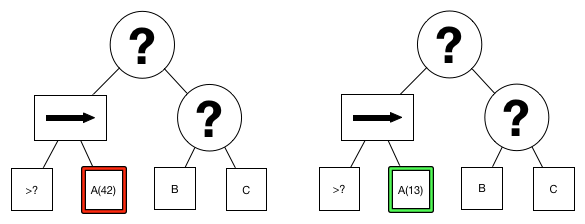
\includegraphics[scale=0.55]{gpmicromutation}
    \caption{Micromutation: choosing a random element in a tree and changing its properties.}
    \label{fig:x gpmicromutationexample}
\end{figure}
\begin{figure}[h]
    \centering
    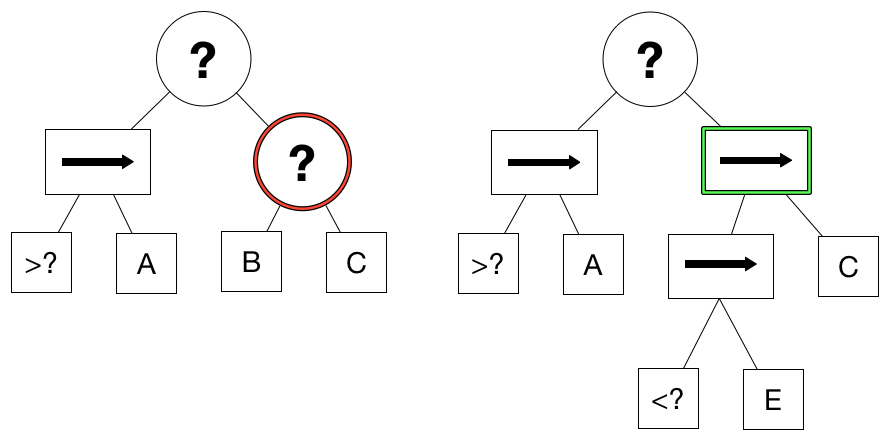
\includegraphics[scale=0.4]{gpmacromutation}
    \caption{Macromutation: after a random node is selected, a new tree is generated and its contents replace selected node.}
    \label{fig:x gpmacromutationexample}
\end{figure}
